\documentclass[a4paper,12pt,onecolumn,twoside]{article}
\usepackage{cite}%bibTeX引用
\usepackage{ctex}
\usepackage{hyperref}%加入超链接
\usepackage{comment}
\usepackage{wrapfig}
\usepackage{graphicx}
\usepackage{float} 
\usepackage{amsmath}
\usepackage{amssymb}
\usepackage{geometry}
\geometry{a4paper,scale=0.8}
\usepackage{float}
\usepackage{subfigure} 
\usepackage{enumerate}%\item 需要
\usepackage{tabularx}% \table 
\usepackage{booktabs}% 	\toprule

%%带颜色的表格%%
%\usepackage[table]{xcolor}
\usepackage{colortbl}
\definecolor{mygray}{gray}{.9}
\definecolor{mypink}{rgb}{.99,.91,.95}
\definecolor{mycyan}{cmyk}{.3,0,0,0}
%%带颜色的表格%%
%%附录代码显示%%
\usepackage{listings}
\usepackage[svgnames]{xcolor}
\lstset{language=R,
	basicstyle=\small\ttfamily,
	stringstyle=\color{DarkGreen},
	otherkeywords={0,1,2,3,4,5,6,7,8,9},
	morekeywords={TRUE,FALSE},
	deletekeywords={data,frame,length,as,character},
	keywordstyle=\color{blue},
	commentstyle=\color{DarkGreen},
}

%%附录代码显示%%
%opening

\begin{document}
\begin{center}
	\Large\heiti{利用一类基于似然函数的时变再生数模型分析2022上海疫情}
\end{center}
\begin{abstract}
	2022年3月,上海发生了冠状病毒聚集性疫情,对全国经济以及居民生活产生了巨大影响。本文介绍了通过基于似然函数的Wallinga-Teunis算法,以及基于此算法开发的R包EpiEstim,通过上海疫情每日新增病例数计算时变再生数的估计值,根据其峰值出现时间,推测疫情发展的最高潮大约在2022年3月20日前后;以其是否降至1以下为标准,推测上海该次疫情的拐点大约为2022年4月18日。\\
	\text{\heiti{关键字:}}2022上海疫情;新型冠状病毒;时变再生数;似然函数
\end{abstract}
\section{问题背景}
2022年2月28日,一位56岁女性因发热前往同济医院发热门诊就诊,核酸检测结果为阳性,并于3月1日复核确诊,成为2022年上海疫情的首个确诊病例。此轮疫情由传染力极强的奥密克戎变异株引发,是上海传播范围最广、感染人数最多的一波冠状病毒病聚集性疫情,呈多点散发、多链并行、隐匿传播、快速蔓延态势,出现了较多的社区传播。4月30日到5月5日,虽然全国日均新增报告感染者近5800余例,但较高峰期已下降80\%。推测疫情拐点出现在四月中旬到五月上旬。
\section{问题分析}
要判断疫情拐点,我们需要找到在何时疫情的传播得到了控制。通常,用以评估某传染病的传染力及疫情严重程度的指标为再生数。下面将介绍本文主要讨论的三种再生数。
\subsection{三种再生数的定义}
\paragraph{基本再生数~}记作$R_{0}$。它的定义是在一个人群中,每一个患原发性疾病的人能够传染的人数。显然,根据定义,当$R_{0}\geq1$时,表明疫情呈发展态势。若已知感染者每单位时间产生的平均感染接触率和平均感染期,则$R_{0}$可表示为两者相乘。平均感染期是由病原体本身决定的,因此这个公式也表明,降低基本再生数的主要方式是减少感染者与其他易感人群的接触频率。
\paragraph{有效再生数~}记作$R_{e}$。通常人群中不全是对某种病原体的易感人群,因此用$R_{0}$乘以易感人群在人群中的比例系数得到$R_{e}$。
\paragraph{时变再生数~}记作$R_{t}$。通常疫情的发展情况是会随着时间变化的,无论是出于其病原体本身的变异还是出于易感人群获得免疫力。因此,引入时变再生数$R_{t}$作为衡量疫情实时可传播性的依据。它代表某一时刻t确诊的一位感染者在其感染期内平均会传染多少人。当时变再生数小于等于1时,代表一个患者平均传染的人数小于1,即疫情得到了控制。
\subsection{隔室模型的不便之处}
一类可用于计算再生数的模型为隔室模型。其中SIR模型是一种常用于分析具有强传染力的传染病的隔室模型,它将人群分配到不同的隔室中,如S(易感),I(已感染),R(已恢复),它们的顺序表示隔室的流动模式,即人群从易感到感染,再到康复。后来有人提出了考虑潜伏期的SEIR模型,其中加入了E(暴露)隔室,还有人提出了SEIS模型,即感染后康复又变为易感人群。\par 
隔室模型的建立和求解一般需要借助微分方程。以新冠肺炎疫情为例,比较适用的模型为SEIR,若使用它来拟合疫情数据,则$R_{e}$的计算方式为
$$R_{e}=(1+\frac{r}{b_{E}})(1+\frac{r}{b_{I}})$$
其中$r$为病例数的增长速率,$b_{E}$,$b_{I}$ 代表E、I两隔室的移出率。如果只研究某医院或某小区新冠疫情的传播,这些数据可以直接根据病人的信息获得。然而当考察的人群庞大时,我们通常是很难获得这些数据的。因此,需要其它的方法来计算再生数。
\subsection{Wallinga-Teunis方法}
Wallinga和Teunis在2004年开发了一种基于似然的估计算法\cite{10.1093/aje/kwh255}。后续,基于该算法,Anne Cori等人开发了R包“EpiEstim”和测试中的应用程序\cite{10.1093/aje/kwt133},可以根据每日新增病例数估计$R_{t}$的动态取值。在后文中,我们也将直接调用该R包来计算2022年初上海疫情的$R_{t}$值。
\section{数据来源}
本文使用的每日新增病例数据来源于Shanghai COVID-19 Reopen项目,项目旨在收集、分享、和可视化由上海市卫健委发布的最新数据。参与计算的数据见附录1.\par 
访问网站:\href{http://reopen.baiyulan.org.cn/}{http://reopen.baiyulan.org.cn/}
\section{模型假设}
我们假设,本文从上海疫情数据公开项目获得的数据是真实可信的,且阳性检出人数即为当日所有的病例数。
\section{符号说明}
\begin{table}[H]
	\centering
	\setlength{\abovecaptionskip}{0pt}%    
	\setlength{\belowcaptionskip}{5pt}%
	\setlength{\tabcolsep}{16mm}
	\caption{符号说明}\label{y}
	\begin{tabular}{cc}
		\toprule
		符号 & 说明                                        \\ \midrule
		$R_{t}$     & 第$t$天的时变再生数             \\
		$n$         & 确诊病例数             \\
		$\lambda$     	& 平均感染率           \\
		$\gamma$    &平均感染期的倒数 \\\midrule
	\end{tabular}
\end{table}

\section{建立模型}
\subsection{基于Wallinga-Teunis方法的时变再生数模型}
一般可以使用泊松分布来拟合传染病的感染过程。假设每天的平均感染率为$\lambda$,则任意一天观察到的确诊病例数$n$的概率分布为:
\begin{equation}
	P(n|\lambda)=\frac{\lambda^{n}e^{-\lambda}}{n!}
\end{equation}
那么,当已知某一天的确诊病例数$n$时,平均感染率$\lambda$分布的似然函数也可表示为
\begin{equation}
	L(\lambda|n)=\frac{\lambda^{n}e^{-\lambda}}{n!}
\end{equation}
而根据Luis M. A. Bettencourt等人的研究\cite{chowell2007comparative},借助SIR模型,可得出$\lambda$和相邻两次汇报的感染人数,与时变再生数$R_{t}$的关系,为
\begin{equation}
	\lambda=e^{\tau\gamma(R_{t}-1)}\Delta n_{t}
\end{equation}
其中,$\gamma$为平均感染期的倒数,$\tau$为病例的汇报间隔。在上海例的数据中,新增病例为每日更新数据,因此$\tau=1.$ 而$\Delta n_{t}$被定义为
\begin{equation}
	\Delta n_{t}=n_{t}-n_{t-\tau}
\end{equation}
根据(2) (3)两式,就得到某相邻两天(即$\tau=1$的情况)新增病例数时,$R_{t}$分布的似然函数。实际操作中,为了将更多的信息利用起来,采取选定的时间窗口来计算$R_{t}$的分布,即某一天的再生数的获得需要其相邻几天的每日新增病例数,选取的时间段称为一个时间窗口。根据Anne Cori等人在其文章附录中的记录,在其正文中,$R_{t}$的先验分布被假设为参数为$(1,5)$的Gamma分布,则其后验分布的任何期望都变得简单易算。详细的推导过程可参见附件(kwt133supp.doc)中的第二节。
\subsection{时间窗口的选择}
在实际操作中,如果数据的时间步长很小,$R_{t}$的估计值会变得不稳定,导致很难用于预测。而对于确诊病例较多的情况,使用W-T方法估计的$R_{t}$值会更高。根据研究,当总共观察到12个(即初始病例+11个)病例后,才开始使用W-T方法估计。事实上,要达成这一条件是很简单的,因为一流行病倘若被发现,其病例数一定已经达到了一定的数量。但对于本文使用的上海疫情数据,到了疫情发展后期时,病例数已经大大减少。在计算中我们将展示如果在确诊病例较少的情况下使用W-T方法将产生怎样的后果。
\subsection{实例计算}
在本节中,参与计算的数据为上海市2022年3月9日至2022年6月24日(日新增首次达到0的日期)的每日新增病例数据,采用一周滑动窗口。原始数据见附录1,计算代码见附录2.~结果如下图所示:
\begin{figure}[H]
	\centering
	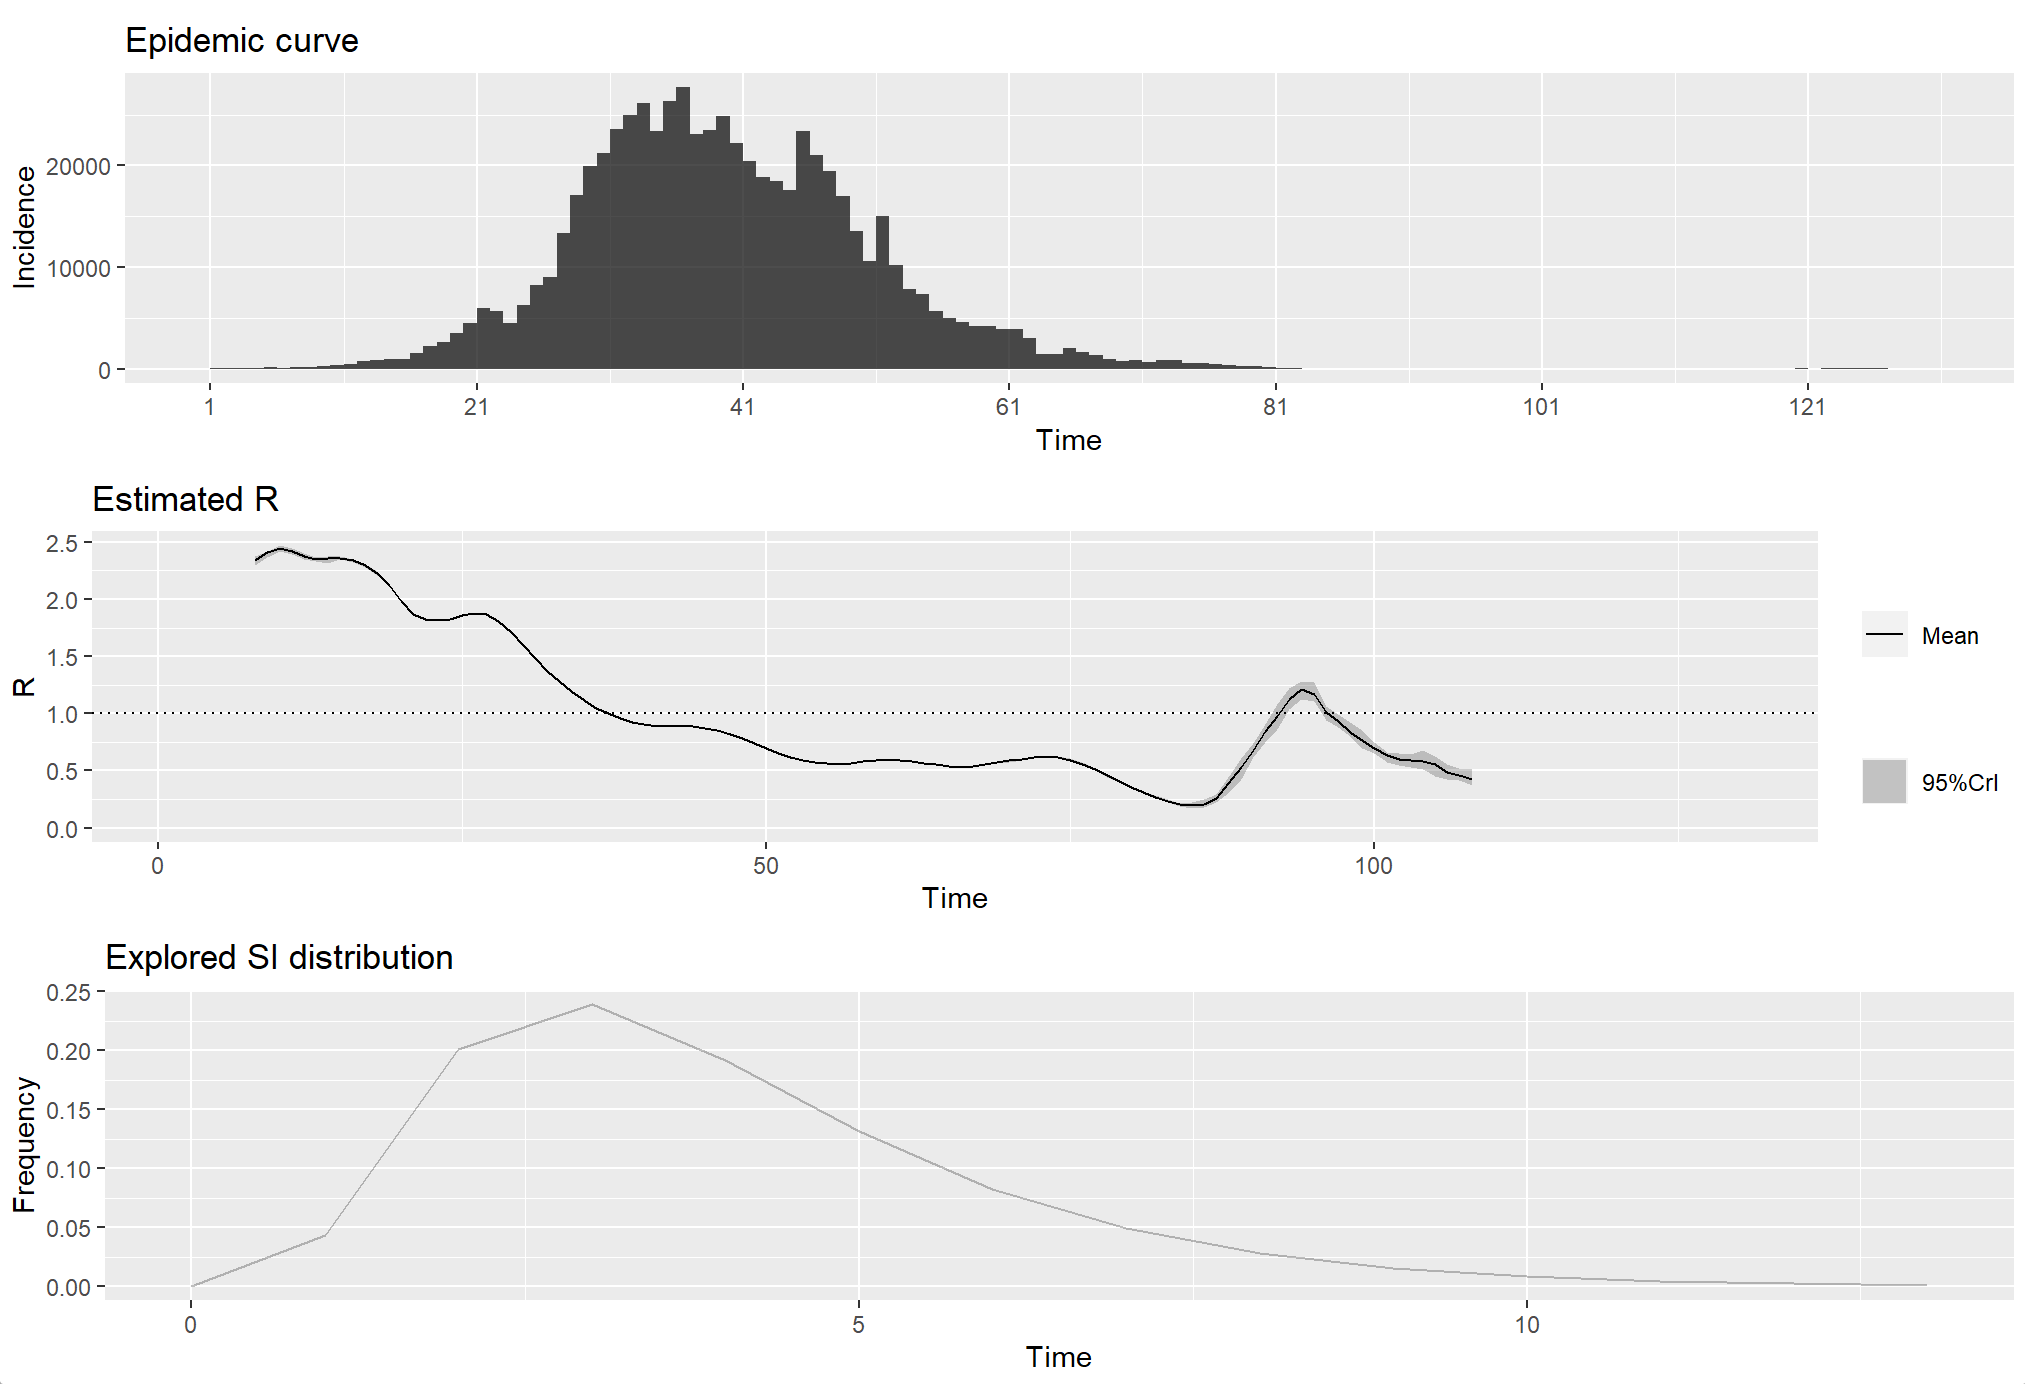
\includegraphics[width=\linewidth]{res/shanghai.png}
	\caption{计算结果}
\end{figure}
从上至下依次为:每日新增数的柱状图,$R_{t}$的变化,序列间隔的分布。序列间隔被定义为一个病例从被感染到其感染别人之间的时间间隔,算法中假设其服从Gamma分布,根据相关流行病学调查研究,新冠病毒的序列间隔均值为4天,标准差为2天。\par 
图中显示,在2022年3月20日前后,$R_{t}$达到了最高值,表示此时一个患者传染的二级患者人数最多,是疫情发展最迅速的时期。大约在2022年4月18日前后,上海疫情的$R_{t}$值降至1以下,这表示在这个时期上海疫情得到缓和。\par 
前文提到,当每日新增病例数过少时,不宜使用W-T方法对$R_{t}$进行估计。而在本例中,上海疫情后期病例大大减少,只有散发病例。上述的计算为了保证模型正确性,刻意避开了这些日期,倘若将这些日期加入计算,我们会发现$R_{t}$的估计值发生了极大的变化:
\begin{figure}[H]
	\centering
	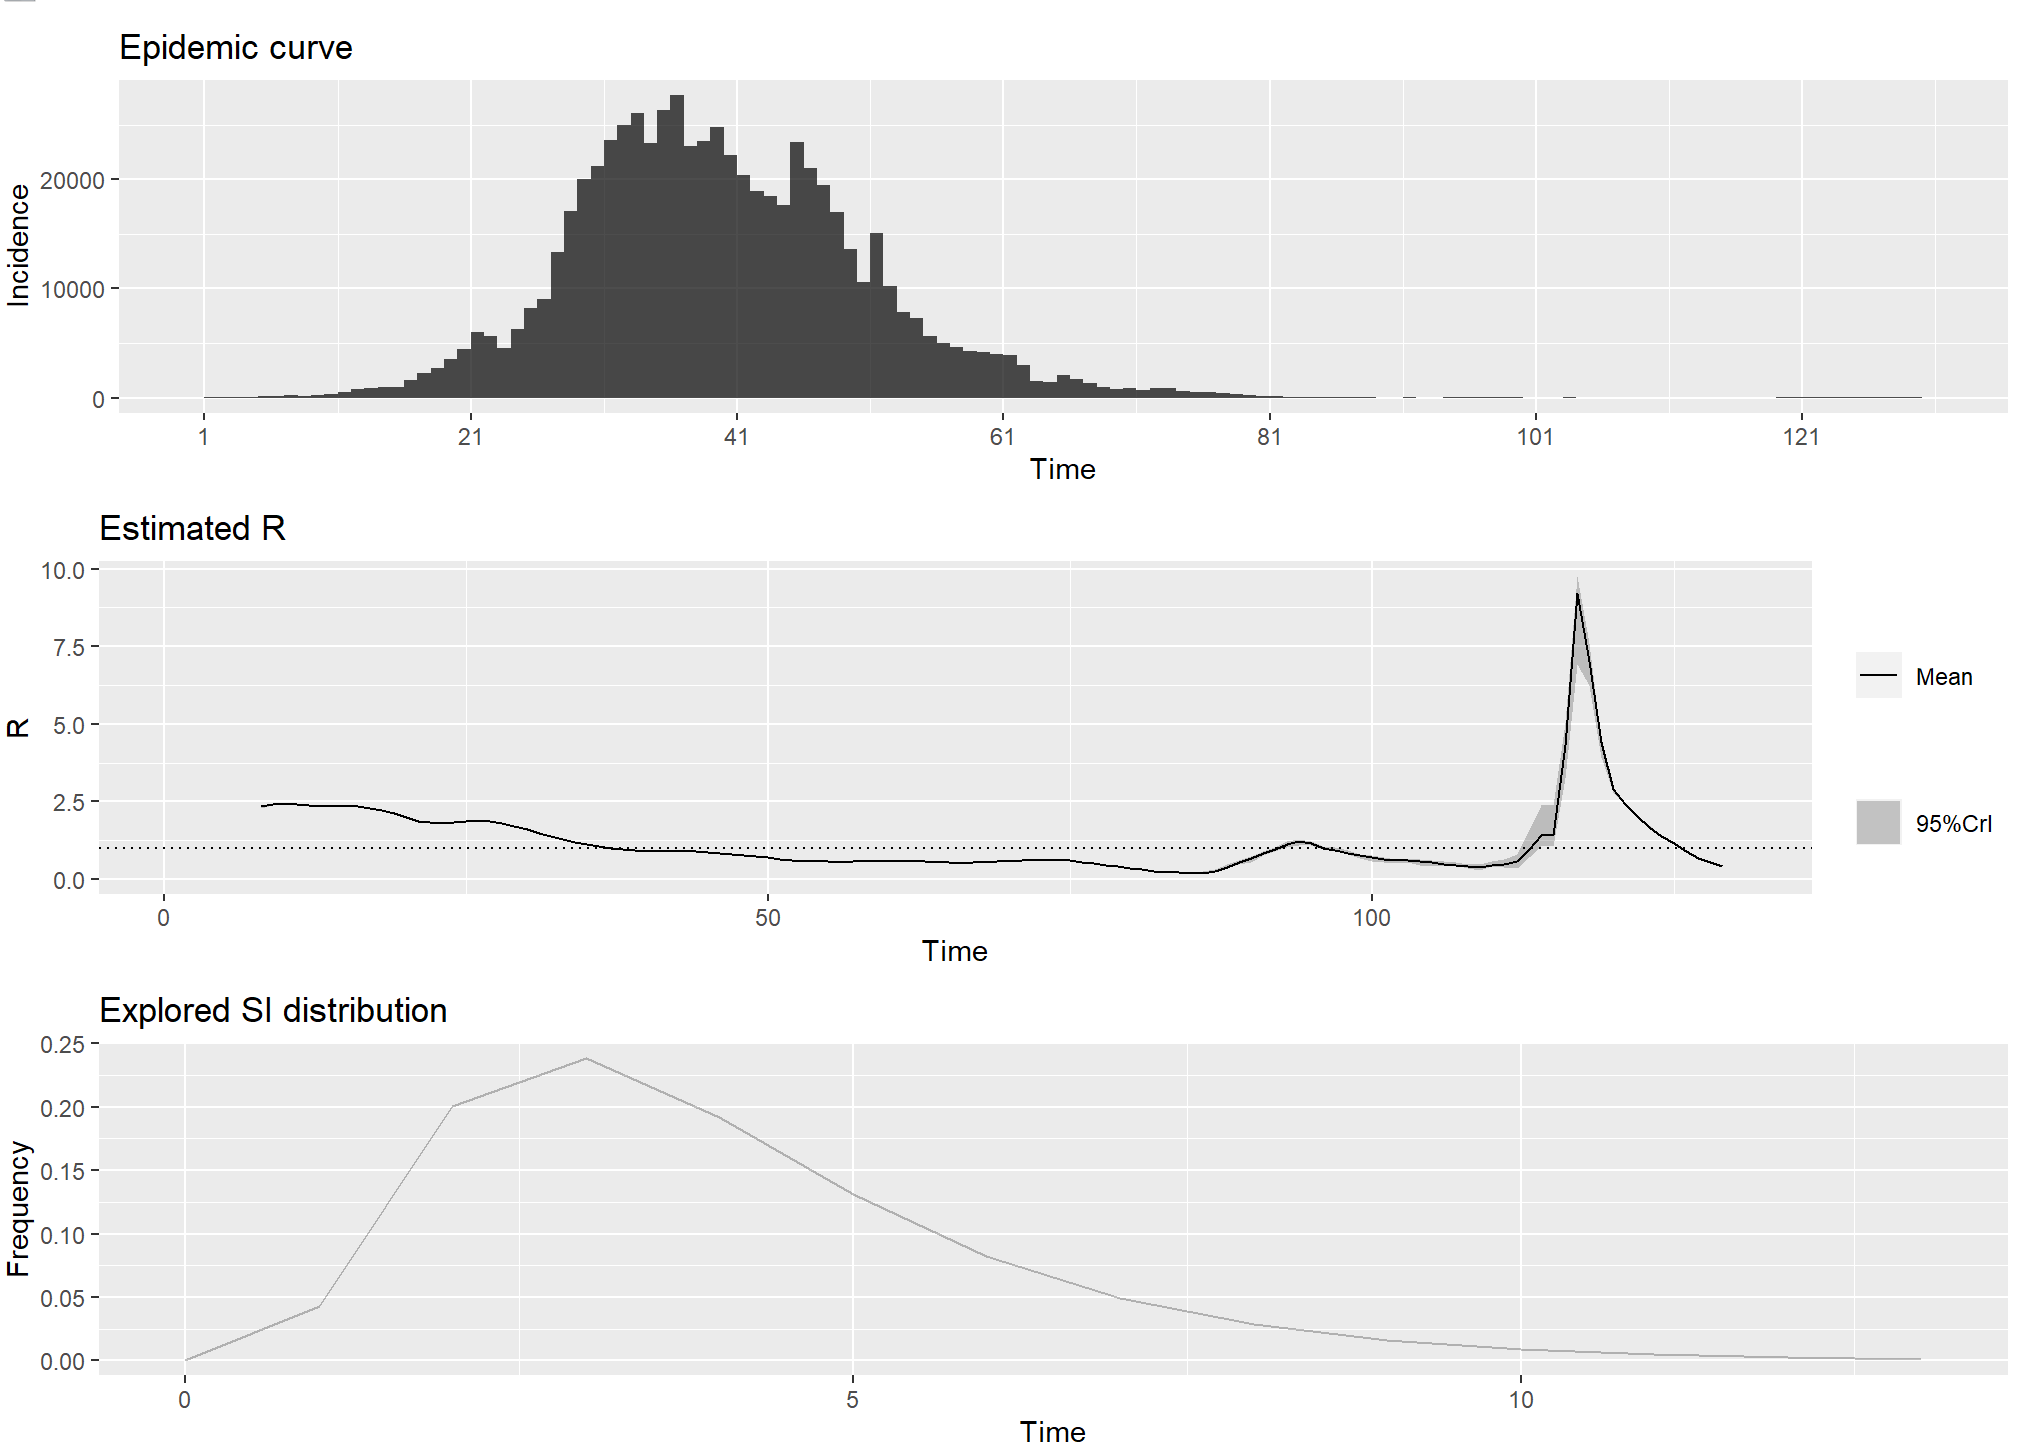
\includegraphics[width=\linewidth]{res/false.png}
	\caption{纳入不合适的日期数据进行计算后产生的结果}
\end{figure}
由图可见,在7月左右,每日新增只有数十人,但使用W-T方法得到的$R_{t}$估计值却几乎接近10,比疫情最严重的三月还要高两倍左右。这是因为时间窗口滑动至每日新增只有0的日期时,由于其不符合每日新增至少为12的条件,产生的计算错误。因此,在使用该算法时,应当尤其注意时间窗口的选择,或可分段进行估算。
\section{模型评价}
\subsection{优点~}诚然隔室模型如SEIR等对疫情的解释是更加合理的,因为它考虑到了更多和疫情发展有直接因果关系的因素。然而在大部分情况下,想要应用隔室模型的条件是严苛的,很多时候甚至需要在没有确切信息来源的情况下凭经验确定某些参数的值,这样反而损伤了模型的合理性。本文介绍的算法应用条件很低,仅需要知道每日新增病例数就可以计算出$R_{t}$的估计值,从而对疫情之后的发展作出预测。
\subsection{缺点~}如6.3所示,该算法对时间窗口的选择敏感,如果有不符合条件的数据参与计算,可能得出荒谬的结果。此外,由于模型需要预先得知每日新增病例数才能对时变再生数$R_{t}$进行估计,因此模型的预报作用相当有限,更多地是用于对疫情的发展情况作出评价。

\addcontentsline{toc}{section}{References}
	\bibliographystyle{IEEEtran}
	\bibliography{cite}

\section*{附录1:参与计算的数据}\addcontentsline{toc}{section}{附录1:参与计算的数据}
\begin{table}[H]
	\centering
	\begin{tabular}{ll|ll|ll|ll} 
		\hline
		date    & cases & date    & cases & date    & cases & date    & cases  \\ 
		\hline
		3/9/22  & 80    & 4/5/22  & 17077 & 5/2/22  & 5669  & 5/29/22 & 67     \\
		3/10/22 & 75    & 4/6/22  & 19982 & 5/3/22  & 4982  & 5/30/22 & 31     \\
		3/11/22 & 83    & 4/7/22  & 21222 & 5/4/22  & 4651  & 5/31/22 & 15     \\
		3/12/22 & 65    & 4/8/22  & 23624 & 5/5/22  & 4269  & 6/1/22  & 13     \\
		3/13/22 & 169   & 4/9/22  & 24943 & 5/6/22  & 4214  & 6/2/22  & 16     \\
		3/14/22 & 139   & 4/10/22 & 26087 & 5/7/22  & 3975  & 6/3/22  & 14     \\
		3/15/22 & 201   & 4/11/22 & 23342 & 5/8/22  & 3947  & 6/4/22  & 22     \\
		3/16/22 & 158   & 4/12/22 & 26330 & 5/9/22  & 3014  & 6/5/22  & 8      \\
		3/17/22 & 260   & 4/13/22 & 27719 & 5/10/22 & 1487  & 6/6/22  & 10     \\
		3/18/22 & 374   & 4/14/22 & 23072 & 5/11/22 & 1449  & 6/7/22  & 15     \\
		3/19/22 & 509   & 4/15/22 & 23513 & 5/12/22 & 2096  & 6/8/22  & 9      \\
		3/20/22 & 758   & 4/16/22 & 24820 & 5/13/22 & 1681  & 6/9/22  & 11     \\
		3/21/22 & 896   & 4/17/22 & 22248 & 5/14/22 & 1369  & 6/10/22 & 16     \\
		3/22/22 & 981   & 4/18/22 & 20416 & 5/15/22 & 938   & 6/11/22 & 29     \\
		3/23/22 & 983   & 4/19/22 & 18901 & 5/16/22 & 823   & 6/12/22 & 37     \\
		3/24/22 & 1609  & 4/20/22 & 18495 & 5/17/22 & 855   & 6/13/22 & 17     \\
		3/25/22 & 2269  & 4/21/22 & 17629 & 5/18/22 & 719   & 6/14/22 & 15     \\
		3/26/22 & 2676  & 4/22/22 & 23370 & 5/19/22 & 858   & 6/15/22 & 16     \\
		3/27/22 & 3500  & 4/23/22 & 21058 & 5/20/22 & 868   & 6/16/22 & 4      \\
		3/28/22 & 4477  & 4/24/22 & 19455 & 5/21/22 & 622   & 6/17/22 & 7      \\
		3/29/22 & 5982  & 4/25/22 & 16980 & 5/22/22 & 558   & 6/18/22 & 9      \\
		3/30/22 & 5653  & 4/26/22 & 13562 & 5/23/22 & 480   & 6/19/22 & 13     \\
		3/31/22 & 4502  & 4/27/22 & 10622 & 5/24/22 & 387   & 6/20/22 & 9      \\
		4/1/22  & 6311  & 4/28/22 & 15032 & 5/25/22 & 338   & 6/21/22 & 8      \\
		4/2/22  & 8226  & 4/29/22 & 10181 & 5/26/22 & 264   & 6/22/22 & 9      \\
		4/3/22  & 9006  & 4/30/22 & 7872  & 5/27/22 & 170   & 6/23/22 & 3      \\
		4/4/22  & 13354 & 5/1/22  & 7333  & 5/28/22 & 122   & 6/24/22 & 0      \\
		\hline
	\end{tabular}
\end{table}

\section*{附录2:计算代码}\addcontentsline{toc}{section}{附录2:计算代码}
\begin{lstlisting}[language=R]
library(tidyverse)
library(EpiEstim)
library(patchwork)
## load data
case.asym.wider.sh<-read.csv('https://raw.githubusercontent.com/
shalom-lab/covid.sh/main/local/share/case.asym.wider.sh.csv')

cases <- case.asym.wider.sh %>%
select(date,pos) %>%
mutate(date=as.Date(date)) %>%
rename(I=pos,date=date)

## wallinga-teunis method to estimate rt
res <- wallinga_teunis(
cases,
method = "parametric_si",
config = make_config(
t_start = seq(1,102),
t_end = seq(7,108),
mean_si = 4, std_si = 2))

plot(res)

\end{lstlisting}

\end{document}
